% CSC209 Assignment 3 -- project.pdf source
% Build: pdflatex report.tex (run twice if references warn)
% Fill \teamname, \members, and Section~\ref{sec:contributions} before submission.

\documentclass[11pt]{article}
\usepackage[margin=1in]{geometry}
\usepackage[T1]{fontenc}
\usepackage[utf8]{inputenc}
\usepackage{microtype}
\usepackage{booktabs}
\usepackage{tabularx}
\usepackage{graphicx}
\usepackage{hyperref}
\usepackage{tikz}
\usetikzlibrary{arrows.meta,positioning}
\usepackage{listings}
\usepackage{caption}

\hypersetup{colorlinks=true, linkcolor=blue, urlcolor=blue, citecolor=blue}

\lstset{
  basicstyle=\ttfamily\small,
  breaklines=true,
  frame=single,
  columns=fullflexible,
  showstringspaces=false
}

\newcommand{\teamname}{\textit{\textless team name on MarkUs\textgreater}}
\newcommand{\members}{\textit{\textless name, student number\textgreater\ (repeat per member)}}

\title{CSC209 Assignment 3\\Multi-Process Monte Carlo $\pi$ Estimator (Pipes)}
\author{\teamname\\\members}
\date{\today}

\begin{document}
\maketitle

% ---------------------------------------------------------------------------
\section{Project Overview}
\label{sec:overview}

\subsection{Category and purpose}
This project is a \textbf{Category~1} systems program: a parent \emph{controller} process coordinates multiple \emph{worker} child processes using \textbf{pipes} for all substantive inter-process communication. The application domain is a Monte Carlo estimator for $\pi$: workers draw uniform random points in $[0,1)^2$ and count hits under $x^2+y^2\le 1$; the controller aggregates hits and trials and reports an estimate, a normal-approximation 95\% confidence interval, and error versus \texttt{M\_PI}.

The emphasis is on \textbf{process orchestration}, \textbf{typed binary protocols}, \textbf{concurrency}, and \textbf{robustness}---not on algorithmic novelty.

\subsection{User interaction}
The controller reads commands from standard input:
\begin{itemize}
  \item \texttt{simulate <N>} --- run $N$ trials across alive workers (work is split and results may arrive in \textbf{multiple partial messages} per worker).
  \item \texttt{setbatch <N>} --- set the maximum trials per partial \texttt{RESULT\_SIMULATE} message (increases message \emph{frequency} for the same $N$ when batches are small).
  \item \texttt{stats} --- query each worker's cumulative simulate-task counter (separate control-plane traffic).
  \item \texttt{workers} --- print alive worker count.
  \item \texttt{help} / \texttt{quit} (or \texttt{exit}).
\end{itemize}

\subsection{Why this satisfies ``communication complexity''}
The wire format is not a single opaque payload per job. The design exposes:
\begin{itemize}
  \item \textbf{Multiple message types} (simulate, status, shutdown, error responses).
  \item \textbf{Versioned structs} (\texttt{PROTOCOL\_VERSION}) so both ends agree on layout and semantics.
  \item \textbf{High-frequency exchanges} when batch sizes are small: one simulate command triggers many \texttt{RESULT\_SIMULATE} messages.
  \item \textbf{Explicit batch metadata} (\texttt{batch\_index}, \texttt{batch\_total}) so the controller can validate ordering and completeness.
\end{itemize}

\subsection{Mathematical note}
For uniform samples in the unit square, the quarter-disk area is $\pi/4$, so $\hat{\pi} \approx 4\cdot(\mathrm{hits}/\mathrm{trials})$.

% ---------------------------------------------------------------------------
\section{Build and run instructions}
\label{sec:build}

\subsection{Environment}
\begin{itemize}
  \item Language: C (GNU/Linux, e.g.\ \texttt{teach.cs}).
  \item Compiler: \texttt{gcc}; build: \texttt{make}.
  \item Flags: \texttt{-Wall -Wextra -g}; link math: \texttt{-lm} for \texttt{controller}.
  \item No third-party libraries beyond the standard toolchain.
\end{itemize}

\subsection{Commands}
\begin{lstlisting}[language=bash]
make clean
make
./controller [num_workers [seed]]
\end{lstlisting}
Defaults: four workers, base seed $42$. Constraints: \texttt{num\_workers} $\in [3,64]$.

\subsection{Typical session}
\begin{lstlisting}[language=bash]
./controller 4 42
# then at the prompt:
help
stats
setbatch 20000
simulate 500000
workers
quit
\end{lstlisting}

\subsection{Optional demo script}
\texttt{demo\_error.sh} rebuilds the project, runs the controller with piped input, kills one worker, and shows that later \texttt{simulate} commands still succeed with fewer alive workers.

\subsection{Note on timing metrics}
The controller prints wall-clock duration and throughput using \texttt{clock\_gettime(CLOCK\_MONOTONIC, ...)}. This is an \textbf{optional observability aid}; core grading mechanisms remain \texttt{fork}, \texttt{exec}, \texttt{pipe}, \texttt{read}/\texttt{write}, \texttt{waitpid}, and signals.

% ---------------------------------------------------------------------------
\section{Architecture}
\label{sec:arch}

Figure~\ref{fig:arch} shows processes and pipes. Each worker has two dedicated unidirectional pipes: \textbf{task} (controller$\rightarrow$worker) and \textbf{result} (worker$\rightarrow$controller).

\begin{figure}[ht]
  \centering
  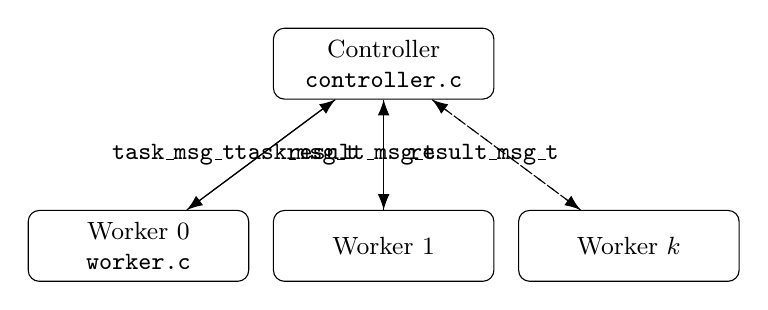
\begin{tikzpicture}[
    proc/.style={draw, rounded corners, minimum width=2.8cm, minimum height=0.9cm, align=center},
    font=\small
  ]
    \node[proc] (ctrl) {Controller\\\texttt{controller.c}};
    \node[proc, below left=1.4cm and 0.3cm of ctrl] (w0) {Worker 0\\\texttt{worker.c}};
    \node[proc, below=1.4cm of ctrl] (w1) {Worker 1};
    \node[proc, below right=1.4cm and 0.3cm of ctrl] (wk) {Worker $k$};
    \draw[-{Latex[length=2mm]}] (ctrl) -- node[left, xshift=-2mm, align=right] {\texttt{task\_msg\_t}} (w0);
    \draw[-{Latex[length=2mm]}] (w0) -- node[right, xshift=2mm, align=left] {\texttt{result\_msg\_t}} (ctrl);
    \draw[-{Latex[length=2mm]}] (ctrl) -- node[left, xshift=-2mm] {\texttt{task\_msg\_t}} (w1);
    \draw[-{Latex[length=2mm]}] (w1) -- node[right, xshift=2mm] {\texttt{result\_msg\_t}} (ctrl);
    \draw[-{Latex[length=2mm]}, dashed] (ctrl) -- (wk);
    \draw[-{Latex[length=2mm]}, dashed] (wk) -- (ctrl);
  \end{tikzpicture}
  \caption{Worker pool: one controller, $N$ workers, two pipes per worker.}
  \label{fig:arch}
\end{figure}

\subsection{Key source files}
\begin{tabularx}{\linewidth}{lX}
  \toprule
  File & Role \\
  \midrule
  \texttt{montecarlo.h} & Shared protocol constants and \texttt{task\_msg\_t} / \texttt{result\_msg\_t}. \\
  \texttt{controller.c} & \texttt{spawn\_workers}, \texttt{run\_simulation}, \texttt{query\_worker\_stats}, \texttt{shutdown\_workers}, REPL. \\
  \texttt{worker.c} & Read loop, Monte Carlo trials, batched responses, status/error replies. \\
  \texttt{Makefile} & \texttt{make} builds \texttt{controller} and \texttt{worker} with \texttt{-Wall -Wextra}. \\
  \bottomrule
\end{tabularx}

% ---------------------------------------------------------------------------
\section{Communication protocol}
\label{sec:protocol}

All messages are \textbf{fixed-width binary structs} sent with a single \texttt{write} of \texttt{sizeof(...)} bytes per message. Partial reads are treated as failure. Helpers \texttt{read\_full} and \texttt{write\_full} retry on \texttt{EINTR}.

\subsection{Request: \texorpdfstring{\texttt{task\_msg\_t} (controller $\rightarrow$ worker)}{\texttt{task\_msg\_t} (controller to worker)}}
\begin{lstlisting}
typedef struct {
    uint32_t version;
    uint32_t task_id;
    uint32_t msg_type;
    uint32_t num_trials;
    uint32_t batch_trials;
} task_msg_t;
\end{lstlisting}
\texttt{msg\_type} is one of \texttt{TASK\_SIMULATE}, \texttt{TASK\_STATUS\_REQ}, or \texttt{TASK\_SHUTDOWN}. Fields \texttt{num\_trials} and \texttt{batch\_trials} apply to \texttt{TASK\_SIMULATE} (batch cap for partial results).

\subsection{Response: \texorpdfstring{\texttt{result\_msg\_t} (worker $\rightarrow$ controller)}{\texttt{result\_msg\_t} (worker to controller)}}
\begin{lstlisting}
typedef struct {
    uint32_t version;
    uint32_t task_id;
    uint32_t msg_type;
    uint32_t num_trials;
    uint32_t num_hits;
    uint32_t batch_index;
    uint32_t batch_total;
    uint32_t tasks_completed;
    uint32_t error_code;
} result_msg_t;
\end{lstlisting}
\texttt{msg\_type} is \texttt{RESULT\_SIMULATE}, \texttt{RESULT\_STATUS}, or \texttt{RESULT\_ERROR}. For simulate batches, \texttt{batch\_index} runs $1\ldots\texttt{batch\_total}$; the controller checks monotonicity and that the sum of \texttt{num\_trials} matches the chunk assigned to that worker.

\subsection{Protocol matrix (summary)}
\begin{table}[ht]
  \centering
  \small
  \begin{tabularx}{\linewidth}{l l X}
    \toprule
    Exchange & When & Notes \\
    \midrule
    \texttt{TASK\_SIMULATE} & User \texttt{simulate} & Carries chunk size and \texttt{batch\_trials}. \\
    \texttt{RESULT\_SIMULATE} & Worker computes & One or many per task; includes batch indices. \\
    \texttt{TASK\_STATUS\_REQ} & User \texttt{stats} & Control traffic distinct from simulate. \\
    \texttt{RESULT\_STATUS} & Worker replies & Exposes \texttt{tasks\_completed}. \\
    \texttt{TASK\_SHUTDOWN} & User \texttt{quit} & Clean termination path. \\
    \texttt{RESULT\_ERROR} & Invalid request / version & Worker-side error reporting. \\
    \bottomrule
  \end{tabularx}
\end{table}

\subsection{Invariants}
\begin{itemize}
  \item \texttt{version} must equal \texttt{PROTOCOL\_VERSION} on both sides.
  \item \texttt{task\_id} on responses must match the outstanding request the controller is aggregating.
  \item For \texttt{RESULT\_SIMULATE}: $\texttt{num\_hits} \le \texttt{num\_trials}$; batch metadata must match the expected batch count derived from chunk and \texttt{batch\_trials}.
\end{itemize}

A reader could re-implement the wire protocol from this section plus \texttt{montecarlo.h} without reading the control flow.

% ---------------------------------------------------------------------------
\section{Concurrency model}
\label{sec:concurrency}

\subsection{Worker pool}
The controller calls \texttt{spawn\_workers} before the REPL: it creates two pipes per worker, \texttt{fork}s, and the child \texttt{execl}s \texttt{./worker} with the read end of the task pipe, the write end of the result pipe, and a per-worker seed. This yields \textbf{at least three concurrent workers} whenever \texttt{num\_workers} $\ge 3$ (enforced in \texttt{main}).

\subsection{Synchronisation}
Workers block on \texttt{read} from the task pipe until the controller sends a message---classic producer/consumer synchronisation via the OS pipe buffer.

\subsection{Simulate path}
For \texttt{simulate N}, the controller counts alive workers, partitions $N$ with a remainder distribution, and writes one \texttt{TASK\_SIMULATE} per worker that receives non-zero work. It then reads \texttt{RESULT\_SIMULATE} messages until each worker's assigned trials are fully accounted for. Partial reads or protocol violations mark that worker dead and close its fds so later commands skip broken peers.

\subsection{Relation to assignment wording}
For very small $N$, some workers may be idle for that command; the \textbf{pool remains concurrently resident}. For reasonable $N$, all workers participate, matching the forum clarification that concurrency should hold for non-trivial workloads.

\subsection{Signals}
\texttt{SIGPIPE} is ignored in the controller so broken pipes surface as \texttt{EPIPE} on \texttt{write}. A \texttt{SIGCHLD} handler reaps terminated children with \texttt{waitpid(..., WNOHANG)} and clears \texttt{alive} flags; heavy cleanup uses the same fd helpers as the main line.

% ---------------------------------------------------------------------------
\section{Error handling and robustness}
\label{sec:errors}

\subsection{Case 1: partial startup failure}
If \texttt{pipe} or \texttt{fork} fails mid-\texttt{spawn\_workers}, the controller runs a \textbf{rollback}: closes already-open pipe fds, terminates and reaps any children already created, resets bookkeeping, and returns failure so \texttt{main} exits cleanly. This avoids orphan processes and fd leaks on failed launch.

\subsection{Case 2: broken pipe while dispatching}
If \texttt{write\_full} fails when sending a task (including \texttt{EPIPE}), the controller calls \texttt{mark\_worker\_dead}: clear \texttt{alive} and close that worker's controller-side fds. Other workers continue to serve later \texttt{simulate} and \texttt{stats} commands.

\subsection{Case 3: bad or incomplete results}
Short reads, wrong \texttt{task\_id}, wrong \texttt{msg\_type}, version mismatch, invalid batch metadata, or trial counts exceeding the assigned chunk all trigger the same policy: mark the worker dead, discard bad data, continue aggregation from healthy workers. This prevents one faulty peer from corrupting global statistics.

\subsection{Case 4: unexpected child exit}
The \texttt{SIGCHLD} handler reaps exited workers so they do not linger as zombies during long interactive sessions.

\subsection{Resource management}
\texttt{close\_worker\_fds} and \texttt{mark\_worker\_dead} centralise fd lifecycle. \texttt{shutdown\_workers} sends \texttt{TASK\_SHUTDOWN}, closes fds, and \texttt{waitpid}s each known child. The core path avoids heap allocation, reducing leak surface.

% ---------------------------------------------------------------------------
\section{Team contributions}
\label{sec:contributions}

\textit{Replace this section with one short paragraph per member (name and student number), describing concrete files and responsibilities (e.g.\ protocol design, \texttt{controller.c} orchestration, \texttt{worker.c} batching, Makefile, report, demo script).}

% ---------------------------------------------------------------------------
\section*{Complexity justification (rubric alignment)}
This project keeps the \textbf{application layer} simple (Monte Carlo) so effort concentrates on \textbf{systems programming}: a versioned, multi-type pipe protocol with optional high message frequency (batching + \texttt{setbatch}), explicit shutdown, status queries, startup rollback, signal-aware IO, and graceful degradation when workers die. Together these address the course emphasis on \emph{encoding}, \emph{message diversity}, \emph{exchange frequency}, and \emph{clear sender/receiver roles}.

\end{document}
